\chapter{figo GmbH}
\section{General Information}
 According to Banks Germany\cite{listOfBanks} "The German banking system is divided by three large sectors: private, public, and cooperative. The cooperative sector is represented by 1,144 credit unions and 2 cooperative central banks. The public sector employs 431 savings bank, 10 land banks and other institutions. Private banks represented 4 transnational banks, 42 investment banks, and 176 regional and other banks. There is also operating are 167 registered branches of foreign banks, including 60 investment banks." While introduction of Payment Services Directive (PSD) and PSD2 by European Commission in European Union together with initiatives of  UK Government regarding API provision and standardization have obligated Banks with the implementation of on-line access points to their services\cite{LarsAPI}\cite{TimAPI}\cite{DaveAPI}. Within the Single European Payment Area acceptance of directive by European Bank Authority scheduled within 2017 year\cite{PSD2}.

figo GmbH is a financial technology company with headquarter in Hamburg. It was founded in 2012  with the mission to “build the backbone of next generation financial services"\cite{figoFAQVision}.  Currently, the API is fully functional in Germany, partly in Austria and England.\cite{figoAngel}\cite{figoCB}

Functions available through API:\cite{figoAPI}
\begin{itemize}
	\item Create, Read, Update, Delete Bank account(s);
	\item Read, Update, Delete Bank account(s) transactions;
	\item Create, Read, Update, Delete Bank account(s) standing orders;
	\item Create, Read, Update, Delete Bank account(s) direct debits;
	\item Read, Update  Bank account(s) securities;
	\item Create, Read, Update, Delete Bank payment(s);
\end{itemize}
To see the list of figo's partners and customers with their use-cases please visit \url{http://figo.io/use\_cases.html}.

figo Connect API was created to accelerate innovations in the FinTech area and to allow figo's partners to offer products with real added value\cite{figoFAQWhat}. It enables developers, startups and even banks to connect to every financial service provider. These partners can access every bank account (current, savings, loan, securities, ...), credit card, eWallet and other financial services like PayPal through one single REST-API. \cite{figoFAQWhat}\cite{figoFAQVision}\cite{figoFAQPartners}


%"The Figo GmbH was founded in 2012 and has its headquarters in Hamburg.
%Figo is a modern and safe with the Figo Connect banking as a service ready platform. Developers can integrate into a variety of services and services thanks to Figo very easy and fast online banking. In addition to the retrieval of account balances and transactions in almost all banks, credit cards and services like PayPal, payments on the platform can be initiated. Figo operates the platform in a German bank for the data center and has been with the "Cloud Services Made in Germany awarded" seal."\cite{figoFAQWhat}
%"The current development in the FinTech scene just shows the need for innovation in the field of finance. Too much was thought of in silos in recent years, and products / services have been developed over the customer. This trend reverses itself just around, and we Figo strive in the same direction. For this reason, we have the Figo Connect API in order to accelerate innovation in the FinTech area and want to allow our partners to offer products with real added value."\cite{figoFAQVision}\\
%"Figo is working with a variety of partners. These partners use our API for very different purposes. "\cite{figoFAQPartners}.List of partners of Figo API with their usecases 
%http://figo.io/use\_ cases.html\\

%"figo’s mission is to “build the backbone of next generation financial services”. 

%Our banking API enables developers, startups and even banks to connect to every financial service provider. These partners can access every bank account (current, savings, loan, securities, ...), credit card, eWallet and other financial services through one single REST-API. It is possible to extract account information and initiate bank transfers \& direct debits.
%With our API, old and new players of the financial service industry are able to easily develop and test new services without the inconvenience of connecting to every single bank.

%Currently, the API is fully functional in Germany and partly in Austria (more countries to follow). Please contact us for access to our API."\cite{figoAngel}

%"Our banking API enables developers, startups and even banks to connect to every financial service provider. These partners can access every bank account (current, savings, loan, securities, ...), credit card, eWallet and other financial services through one single REST-API. It is possible to extract account information and initiate bank transfers \& direct debits. With our API, old and new players of the financial service industry are able to easily develop and test new services without the inconvenience of connecting to every single bank."\cite{figoCB}

\section{IT infrastructure. Banking Server}
The high level IT infrastructure of figo GmbH consists two parts (Fig. \ref{fig:figoArch}). The \textbf{API Server} - implements interfaces to figo's customers and partners for accessing banking information and services (lays outside of this paper's scope). The \textbf{Banking Server} - implements connection to banks via three possible communication channels, they are description provided below together with basic motivation for each of them.
\begin{figure}[ht]
  	\label{fig:figoArch}
    \centering
    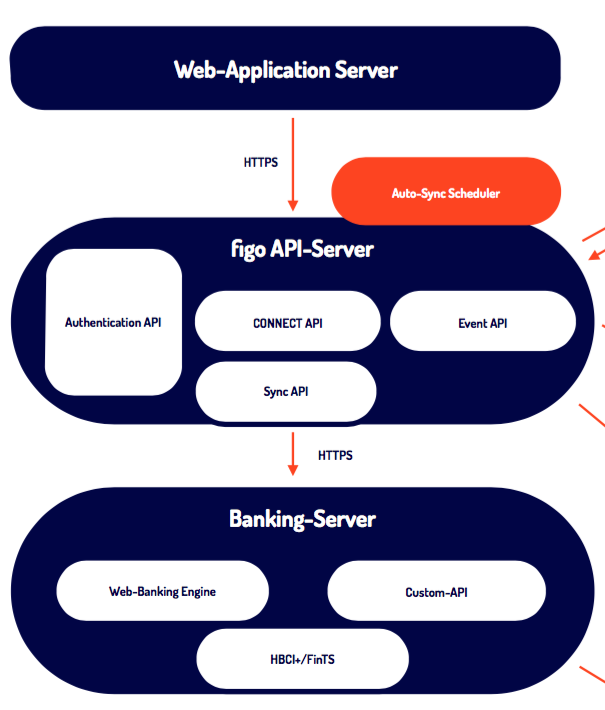
\includegraphics[scale=0.3]{grafiken/figoArch.png}
     \caption{figo GmbH high level architecture}
\end{figure}

\subsection{Banking Server Architecture}
	
	Banking server has three parts for communication with banks via three separate channels. Each of them is a realization of different technology: \textbf{\textit{Custom-API}} is responsible for connection to custom APIs provided by banks, \textbf{\textit{HBCI/FinTS}} is responsible for connection to banks' interfaces via FinTS/HBCI, \textbf{\textit{Web-banking Engine}} is responsible for communication with banks which does not provide API or HBCI.

	\paragraph{Custom-API} implements the client for custom banks APIs. Some of them provide full functionality while some only partial. All this APIs vary in their structure and functionality but most of them implements REST API specification.
	
	\paragraph{HBCI+/FinTS} is an implementation of an adapter OOP pattern for jsHBCI library. Home Banking Computer Interface (HBCI) is an open publicly available protocol. Its specification was originally designed by the two German banking groups \textit{Sparkasse and Volksbanken und Raiffeisenbanken} and \textit{German higher-level associations as the Bundesverband deutscher Banken e.V.}.  \cite{finTS}
	
	\paragraph{Web-Banking Engine} is an implementation of a factory OOP pattern for scraping libraries which responsible for communication with banks which does not provide API or HBCI. Here figo GmbH uses web scraping technology to perform interaction with internet banking web page.
	From the banks perspective an interaction looks completely like direct communication with an user, while an user does not feel the difference between interaction via Custom-API or HBCI or Web-Banking Engine.
	This is the most sensitive part from the developer's perspective since every change to the bank's web page can leads to failure of the specific scripts. \\
	
	The aim of this paper is an application of Test Sheet for early (before any user's interaction will take place) recognition of page changes  and notification of developers regarding failed part of the script. Testing scripts generated from Test Sheets are used as a (demon task/crown job) in timely fashion with notification of the developer in case of unexpected behavior of the scripts via (email/slack) communication channel. 

	
	%\subsection{Banking Technology Stack}
	%banking server only
	
	

